
\exercise{Eigenvector in a Branch}{2}
Suppose the adjacency matrix of the following network has an eigenvalue $\lambda$ with the corresponding eigenvector $\vec{v}$:
\begin{center}
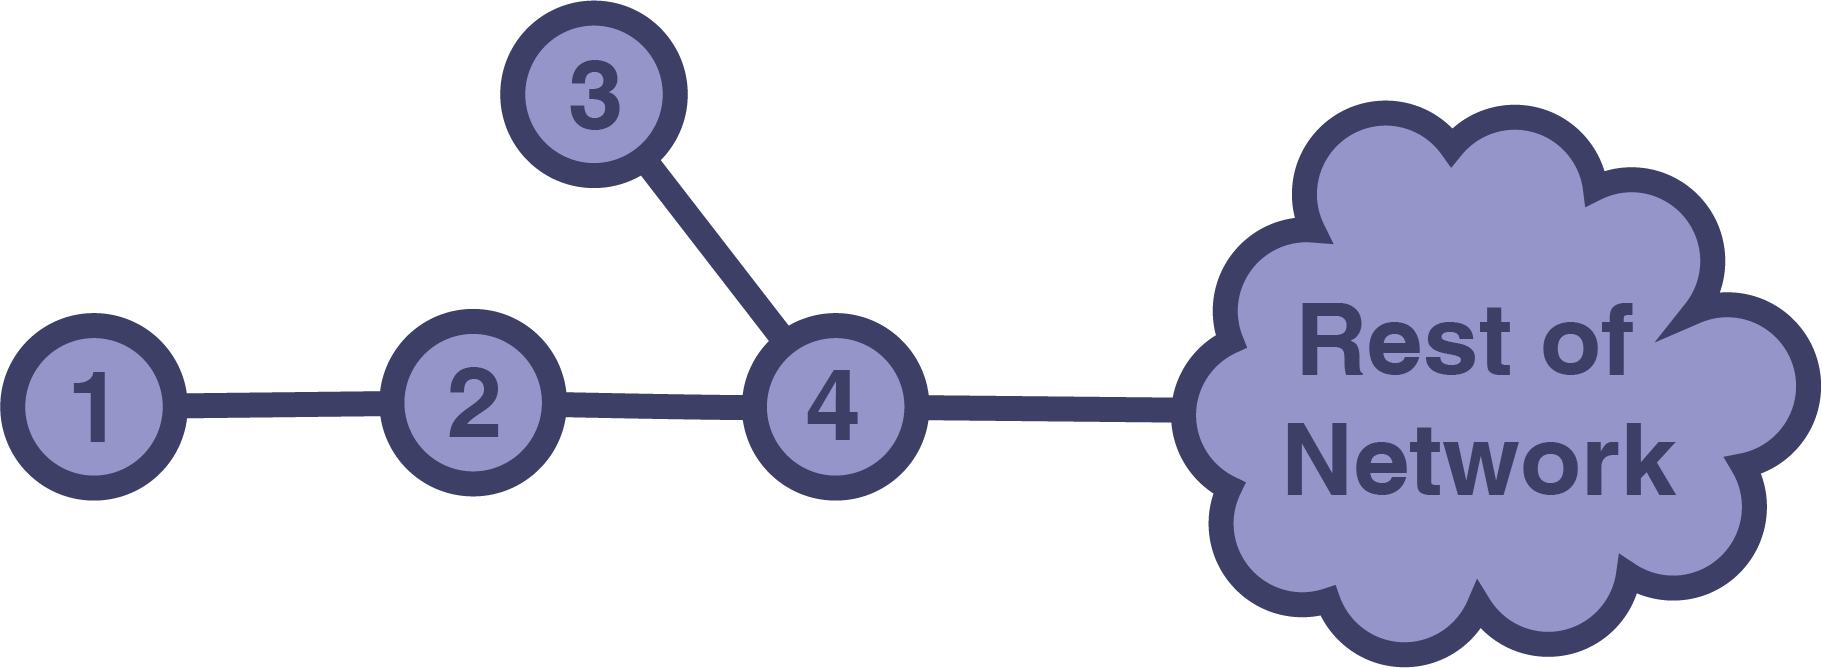
\includegraphics[width=0.4\textwidth]{branch}
\end{center}

\subquestion 
Consider the eigenvector $v_1$ and $v_2$ element of $\vec{v}$ that correspond to node 1 and 2, respectively. Express $v_2$ as a function of $v_1$ and $\lambda$. 

\solution 
We start from the eigenvector equation 
\eq{
{\bf A} \vec{v} = \lambda \vec{v}.
}
Node 1 has only one neighbor, node 2, hence the first row of $\bf A$ only contains one non-zero element, $A_{1,2}=1$. Hence, the first row of the eigenvector equation reads
\eq{
A_{1,2} v_2 = \lambda v_1. 
}
Using $A_{1,2}=1$ we can write this as 
\eq{
v_2 = \lambda v_1.
}

\subquestion 
Also express $v_2$, $v_3$ and $v_4$ as functions of $\lambda$ and $v_1$. 

\solution
The second row of the eigenvector equation reads 
\eq{
A_{1,2}v_1 + A_{2,4} v_4 = \lambda v_2, 
}
and hence 
\eq{
v_1 + v_4 = \lambda v_2
}
We substitute our result for $v_2$ and solve for $v_4$ to find
\eq{
v_4 = (\lambda^2 - 1) v_1 
}

To find $v_3$ we consider the third row of the Eigenvector equation which reads
\eq{
A_{3,4}v_4 = \lambda v_3.
}
Solving for $v_3$ we find
\eq{
v_3 = \frac{v_4}{\lambda} = \frac{\lambda^2 - 1}{\lambda} v_1 
}
Of course if continued this process for the whole network and then set $v_1=1$ the last condition would impose another constraint giving us a self-consistency condition for $\lambda$. This condition is of course the characteristic polynomial (give or take some minor rearrangements). Especially for larger networks it is usually more fun to find the characteristic polynomial this way instead of evaluating a large determinant.   

\subquestion For which values of $\lambda$ would $v_1$ and $v_3$ have the same sign. 

\solution 
Based on the previous result for $v_3$, $v_1$ and $v_3$ have the same sign if 
\eq{
\frac{\lambda^2 - 1}{\lambda} > 0
}
If $\lambda$ is positive this yields the condition
\eq{
\lambda>1
}
For the case $\lambda<0$ is negative we multiply both sides with $\lambda$, 
\eqa{
\lambda^2 -1 &<& \lambda \\
\lambda^2 -\lambda -1 &<& 0 \\
(\lambda -1/2)^2 &<& 5/4 
}
Since we are looking for negative values of $\lambda$ we only need to consider the negative square root, which leads us to the golden ratio's little brother
\eq{
\lambda  > \frac{1-\sqrt{5}}{2}. 
}
In summary, if $\lambda>1$ then $v_1$ and $v_3$ have the same sign. In this case all of the elements of our four nodes will have the same sign. The nodes in this sparsely connected branch find it difficult to sustain large eigenvalues, if other parts of the network want a large eigenvalue our four nodes have to pull all in the same direction to keep up.  

If $0<\lambda<1$ then $v_1$ and $v_3$ have the opposite sign. If we check the other conditions we can see that the sign change occurs between node 3 and node 4. In fact, we elements corresponding to nodes of degree one always have the same sign as their neighbor if $\lambda>0$ and the opposite sign if $\lambda<0$. 

If $(1-\sqrt{5})/2< \lambda < 0$ then $v_1$ and $v_3$ have the same sign, but $v_2$ and $v_3$ now have the opposite sign.  

If $\lambda<(1-\sqrt{5})/2$ then then $v_1$ and $v_3$ have once again the opposite sign. To sustain such a negative eigenvalue the sign now needs to change in every link. So $v_1$ and $v_4$ have the same sign and $v_2$ and $v_3$ have the same sign. 
 



